\cleartooddpage[\thispagestyle{empty}]
\chapter{Introduction}\label{CHAPTER1}

Subarachnoid hemorrhage is a potentially devastating pathologic condition in which bleeding occurs between the brain and the tissues that cover the brain. One of the prevalent pathologic conditions that may result in subarachnoid hemorrhage is the rupture of an intracranial aneurysms (IA). IAs are an irregular expansion of sections of the cerebral vasculature, due to pathologic changes to vascular cells and resulting in an overall weakening of the vascular wall \cite{}.

Research has shown that there a wide array of risk factors may impact IA development and rupture \cite{Korja2014,penn2014role,starke2014tumor,diagbouga2018role}. Quantification of factors contributing to the development and potential rupture of IAs are important to both understand and decrease the risks associated with this potentially life-threatening pathology. Typically, the geometrical properties of vessels and aneurysms have been used as the basis for clinical predictions of aneurysm rupture, subsequently directing the course of clinical intervention(s) \cite{Steiner_2018,Thompson2015guidelines}


Lorem ipsum dolor sit amet, at qui viderer recusabo aliquando, dignissim 
evertitur ei his. Ignota iuvaret fabulas ei vim. Ne utinam inciderint quo. 
Pri ea congue postulant conclusionemque. Ut elitr dicam elaboraret pro, ius 
altera voluptaria cu. Eam mazim aliquip cu, recusabo pericula accommodare at 
mea, facer affert nonumes qui ea.

Discere dissentiet vel et, soluta nostrum epicurei ad eam, cu has aperiam 
vituperata. In prima quaeque diceret pri. Enim labores contentiones eos at, 
duo altera denique nominavi ea, eos inani nominavi consectetuer at. Ut elitr 
dicam elaboraret pro, ius altera voluptaria cu. Eam mazim aliquip cu, 
recusabo pericula accommodare at mea, facer affert nonumes qui ea.
\cite{Crystal09_01,DMOL3_01,HPL_DGEMM_02}

\section{Section 1}\label{CHAPTER1_SECTION1}

At vix indoctum disputando. Eam cu doctus reprimique, quaeque democritum 
an eos, sit veniam facete dissentias id. Tale volumus eos te, an eum nulla 
tincidunt. Mea id recteque theophrastus.

Eirmod malorum vis ei. Choro euismod incorrupte in vim, ludus ornatus vis ex. 
Hinc wisi impedit eum no, vocent definiebas referrentur in quo. Sanctus 
vulputate repudiandae usu ut.

\subsection{Objective}\label{CHAPTER1_SECTION1_SUBSECTION1}

Although there exists a number of studies\cite{can2015association,zhou2017association,varble2018stroke} and methodologies\cite{etminan2015unruptured,greving2014development} that attempt to assess IAs at a high risk of rupture, inconsistencies between study outcomes leave the development of an ideal predictive model out of reach. In addition, many of these previous studies assess the geometric\cite{abboud2017morphology,kashiwazaki2013size,varble2018stroke} and/or hemodynamic wall stressors\cite{zhou2017association,Miura519,can2015association} as a means to predict IA rupture, with limited quantitative assessment of the hemodynamic flow conditions within the aneurysm. \textbf{The primary objective} of this work is to assess the viability of adapting quantitative analysis of hemodynamic flow patterns, specifically swirling flow pattern(s) (vortex), within IAs to improve the prediction and understanding of IA rupture. In this work, an overview of recent theories concerning 

\begin{figure}[htb]
  \begin{center}
    \begin{tikzpicture}[scale=0.60, every node/.style={scale=0.60}]
      \path[mindmap,concept color=Black,text=White]
      node[concept] {\begin{equation*}\sum_{i,j=1}^{M,N}\,\alpha_{ij}\,\beta_{ji}\,=\,?\end{equation*}}
      [clockwise from=0]
      child[concept color=RoyalBlue!65!Black] { node[concept] {A1}
        [clockwise from=90]
        child { node[concept] {ABCD} }
        child { node[concept] {EFGH} }
        child { node[concept] {IJKL} }
      }
      child[concept color=OrangeRed!65!Black] { node[concept] {B2}
        [clockwise from=0]
        child { node[concept] {TUVWX} }
        child { node[concept] {YZABC} }
      }
      child[concept color=DarkGoldenRod!65!Black] { node[concept] {C3}
        [clockwise from=-45]
        child { node[concept] {123} }
        child { node[concept] {789} }
      }
      child[concept color=Plum!65!Black] { node[concept] {D4}
        [clockwise from=-90]
        child { node[concept] {$\alpha$} }
        child { node[concept] {$\beta\,\gamma$} }
        child { node[concept] {$\pi$} }
        child { node[concept] {$\eta$} }
      }
      child[concept color=ForestGreen!65!Black] { node[concept] {$\nabla\,\psi \,=\, \delta\,\phi$}
      }
      child[concept color=LightCoral!65!Black] { node[concept] {\begin{equation*}\int_{0}^{\infty}\,\frac{1}{x}\,dx\end{equation*}}
      } ;
    \end{tikzpicture}
  \end{center}
  \caption{Schematic representation of our universe}
  \label{CHAPTER1_FIG01}
\end{figure}


\subsection{Methodolgy}\label{CHAPTER1_SECTION1_SUBSECTION2}
For the initial focus of this work, image-based computational fluid dynamics models of patient-specific IA geometry will be constructed from 3D phase contrast magnetic resonance imaging (PC-MRI). Computational fluid dynamic (CFD) simulations will be performed on the computational models to generate realistic 3D hemodyanmic velocity and flow pattern data. From said data, 


\begin{figure}[htb]
  \begin{center}
    \begin{tikzpicture}[domain=0:4]
      \draw[very thin,color=gray] (-0.1,-1.1) grid (3.9,3.9);
      \draw[->] (-0.2,0) -- (4.2,0) node[right] {$x$};
      \draw[->] (0,-1.2) -- (0,4.2) node[above] {$f(x)$};
      \draw[color=red] plot[id=x] function{x}
        node[right] {$x$};
      \draw[color=blue] plot[id=sin] function{sin(x)}
        node[right] {$\sin x$};
      \draw[color=orange] plot[id=exp] function{0.05*exp(x)}
        node[right] {$\frac{1}{20} \mathrm e^x$};
    \end{tikzpicture}
  \end{center}
  \caption{Mathematical functions plotted using TikZ package}
  \label{CHAPTER1_FIG02}
\end{figure}

Simul noster voluptaria eam ei, sint regione pri ei. Cum no utinam equidem, 
falli bonorum prodesset an qui. Alterum dissentiet vituperatoribus te eam, 
eos ea suas oblique. Per ea utinam facilisi. \cite{DMOL3_02,HPL_01,HPL_02}
Per iudico probatus complectitur et, cum tollit atomorum rationibus ea.

\section{Aneurysm Geometic Characterisitcs}\label{CHAPTER1_SECTION2}

All aneurysm geometries were taken from the finalized computational mesh generated for simulations. The aneurysm sac was manually isolated from the parent vessel and the resultant cut plane was capped and identified as the IA ostium using an in-house script written in VMTK. Geometric measurements were either taken directly from the values reported in the Aneurisk dataset, or were calculated using in-house scripts in VMTK. 

\underline{Aneurysm Surface Area and Volume}: Measured directly from the isolated IA geometry before and after (respectively) ostium capping. A number of studies have eluded to an increase in IA size as a risk for both IA growth and rupture. \cite{varble2018stroke,brinjikji2015risk,Backes951,greving2014development}. A meta-analysis performed by Brinjikji et al reported that IA $\le$ 10 mm in size (diameter) grew at a rate $<$ 2.9\% per year, while IAs $>$ 10 mm were associated with growth rates of 9.7\% per year. This growth was also reported with an associated IA rupture rate: 3.1\% per year compared with 0.1\% per year for stable (non-growing) aneurysms (p $\le$ 01). From a clinical perspective, the overall size of an aneurysm is often a characteristic used to determine course of IA treatment (or lack thereof) \cite{williams2013management,komotar2008guidelines}. Yet while large IAs are thought to increase the likelihood of rupture, a not-insignificant number of small IAs ($<$5 mm diameter) also have been shown to rupture \cite{kashiwazaki2013size,forget2001review,Korja2014}. This disparity between sizes of ruptured IAs suggest that the assessment of additional factors in tandem with IA size improve rupture prediction. 

\underline{Aneurysm Height}: The length of the centerline of the IA sac is measured, following the IA shape, as opposed to measuring a straight line from the ostium centroid directly to the highest IA point. The radius of the maximum inscribed sphere at the centerline's furthest point is added to the length measurement to fully measure the IA height. This is a modified version of the typical IA height measurement: a straight line of the maximum stretch from the ostium centroid to the IA dome \cite{ma2010size,duan2018morphological}. 

\underline{Vessel Diameter}: The parent artery diameter value is computed at locations close to the aneurysm ostium. For side-wall aneurysms only the location prior to the aneurysm is used. For terminal aneurysms, the vessel diameter along the common branch and both daughter arteries are measured and averaged.

\underline{Inlet Cross-sectional Area}: The beginning of the inlet vessel was cut square in the 3-matic software package, the resultant cross-sectional area of the inlet vessel was calculated. 
 
\underline{Aspect Ratio*}: A modified calculation of the commonly defined aspect ratio (aneurysm hight/ostium diameter) was used adapting the sac centerline (SC) length as a measure of aneurysm height \cite{piccinelli2012characterization}.
\begin{equation}
Aspect Ratio* = (SC_{length} / (4*(Ostium_{area} / Ostium_{circumfrence})))
\end{equation}

\section{Aneurysm Hemodynamic Characterisitcs}\label{CHAPTER1_SECTION3}


\underline{Wall Shear Stress}: 
The calculation of wall shear stress (WSS) is performed by the ANSYS-FLUENT commercial finite-element solver (ANSYS v17.0). The value is defined as the normal velocity gradient against the (vessel) wall:
\begin{equation} \label{WSS}
\tau_w = \mu\frac{\partial v}{\partial n}
\end{equation}
with $\mu$ as the fluid dynamic viscosity (0.004 kg/m-s). 

The spatial-temporally averaged value of the aneurysm's WSS was calculated alongside its temporally-averaged WSS minimum and temporally-averaged WSS maximum. 

\underline{Kinetic Energy Density}:

\section{Disturbed Flow on Vascular Endothelium}\label{Chapter1_Section4}

The vascular endothelial cell (EC) layer forms the innermost lining of blood vessels, directly interacting with hemodynamic stressors and helping to maintain homeostatic functions of the vasculature\cite{chien2007mechanotransduction,gimbrone2016endothelial}. The mechanotransduction capabilities of this initial vascular layer help maintain a selective macromoleuclar barrier, trigger vascular remodeling, regulate vascular smooth muscle cell contraction\cite{vanhoutte2009endothelial}, and help control vascular inflammatory responses\cite{chalouhi2012biology}. The degradation of vascular homeostatsis, resultant from disturbed hemodynamic flow patterns, has been associated with an array of vascular pathologies: aneurysms\cite{Cebral119,LONGO2017632}, atherosclerosis\cite{Liu2015}, and thrombosis\cite{chiu2011effects,uzarski2013adaptation}. Due to the life threating nature of IAs, improved quantitative methods to characterize hemodynamic patterns and to what degree they impart EC pathologic changes, could prove essential to further our understanding of the disease's initiation and progression. 

The morphology and cytoskeletoal organization of EC have been shown to be susceptible to non-laminar flow conditions\cite{wang2013endothelial}. Typically, EC morphology aligns along flow directionality, forming organized parallel actin stress fibers and giving the cells an elongated  
structure\cite{thomas2016biomimetic,gimbrone2016endothelial,balaguru2016disturbed}. Disrupted flow patterns resulting in vortex flow and altered WSS, show a differential change in EC characteristics: a rounded morphology with marginally located short actin stress fibers\cite{chiu2011effects,uzarski2013adaptation,dolan2011high}.


The inflammatory process within vasculature has been shown to be a significant actor in the pathogenesis of IA development and potential rupture \cite{chalouhi2012biology,hashimoto2006,signorelli2018}. In a typical physiological setting, the vascular EC layer maintains antiatherogenic characteristics, inhibiting platelet adhesion and aggregation along the vascular wall, as well as limiting cellular pro-inflammatory pathways\cite{ALSOUDI2017951}. In the occurrence of IA pathology, a breakdown of the EC inflammatory-limiting capabilities is noted: small aneurysm shown to have intimal thickening and diffuse macrophage/lymphocyte infiltration, whereas chronic atherosclerotic lesions with embedded macrophages and lymphocytes have been noted in larger aneurysms\cite{Frösen2012,kosierkiewicz1994}. Upon leukocyte and macrophage infiltration, the matrix metalloproteinase enzyme is released which digests extracellular matrix proteins leading to additional pathologic damage to the vascular wall\cite{tronic2000,aoki2007a}. The remodeling of the vascular wall, impart due to inflammatory pathogenic activities, lead to an overall loss vessel mechanical strength and a possible ballooning out of the impacted area   



Docendi eligendi sit et, pri ea dicam eligendi percipitur, has soleat 
dolores convenire te. Sed altera placerat an, id verterem abhorreant 
interesset mea. Eum at ceteros efficiantur. Eos id voluptaria efficiendi 
comprehensam. \cite{HPL_DGEMM_01,HPL_DGEMM_02}

\begin{figure}[hbt]
  \begin{center}
    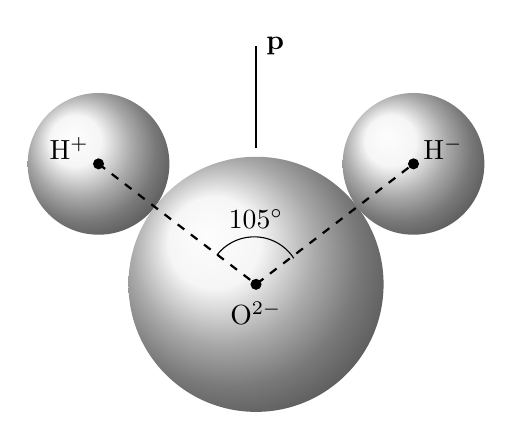
\begin{tikzpicture}[>=latex,scale=1.0]
      \shade[ball color=gray!10!] (0,0) coordinate(Hp) circle (.9) ;
      \shade[ball color=gray!10!] (2,-1.53) coordinate(O) circle (1.62) ;
      \shade[ball color=gray!10!] (4,0) coordinate(Hm) circle (.9) ;
      \draw[thick,dashed] (0,0) -- (2,-1.53) -- (4,0) ;
      \draw[thick] (2,.2) -- (2,1.5) node[right]{$\mathbf{p}$} ;
      \draw (2.48,-1.2) arc (33:142:.6)  ;
      \draw (2,-.95) node[above]{$105^{\circ}$} ;
      \draw (0,.2) node[left]{H$^+$} ;
      \draw (4,.2) node[right]{H$^-$} ;
      \draw (2,-1.63) node[below]{O$^{2-}$} ;
      \foreach \point in {O,Hp,Hm}
        \fill [black] (\point) circle (2pt) ;
    \end{tikzpicture}
  \end{center}
  \caption{Schematic representation of a water molecule}
  \label{CHAPTER1_FIG03}
\end{figure}

In mel modo dicam vocibus, eruditi consectetuer vim no, cu quaestio 
instructior eum. Justo nostrud fuisset ea mea, eam an libris repudiandae 
vituperatoribus. Est choro corrumpit definitionem at. Vel sint adhuc vocibus 
ea, illud epicuri eos no. Sea simul officiis ea, et qui veri invidunt 
appellantur. Vix et eros ancillae pertinax. 
\cite{GROMACS4,GULP_01,GULP_02,HYPRE_01,LAMMPS_01}
Per iudico probatus complectitur et, cum tollit atomorum rationibus ea.
Per iudico probatus complectitur et, cum tollit atomorum rationibus ea.

Aliquip lobortis ei est, at error viris graeco sed. Vel te elitr detracto, 
modo graecis scripserit ex nec. Errem utamur viderer per no, eam ea eripuit 
referrentur. Pro te dicat disputando. Per iudico probatus complectitur et, 
cum tollit atomorum rationibus ea. \cite{R_01,SIESTA_01,SIESTA_02,SMEAGOL_01}.
Per iudico probatus complectitur et, cum tollit atomorum rationibus ea.

Per iudico probatus complectitur et, cum tollit atomorum rationibus ea.
Docendi eligendi sit et, pri ea dicam eligendi percipitur, has soleat 
dolores convenire te. Per iudico probatus complectitur et, cum tollit 
atomorum rationibus ea.
